% =========================================================================
%   Ensuring Functional Equivalence in Retrofitted Anti-Skid Systems
%   for European Public Transportation
%   Author: Mert Torun, M.Sc.
%   Venue:  Kölner Beiträge zur technischen Informatik (ISSN 2193-570X)
% =========================================================================
\documentclass[journal, a4paper]{IEEEtran}

% --- Core Packages ---
\usepackage[T1]{fontenc}
\usepackage{lmodern}
\usepackage[utf8]{inputenc}
\renewcommand{\rmdefault}{lmr}
\renewcommand{\sfdefault}{lmss}
\renewcommand{\ttdefault}{lmtt}
\usepackage{cite}
\usepackage{amsmath}
\usepackage{graphicx}
  \graphicspath{{fig/}}
\usepackage{url}
\usepackage{enumitem}
\usepackage{siunitx}
\usepackage{booktabs}
\usepackage[expansion=false,tracking=true]{microtype}
\setlength{\emergencystretch}{3em}
\hbadness=10000 % suppress cosmetic underfull-hbox warnings (unavoidable in narrow IEEE columns)
\vbadness=10000 % suppress cosmetic underfull-vbox warnings
% No-op revision-tracking macros (retained so any stray markup compiles cleanly).
\newcommand{\reviewcomment}[1]{}
\newcommand{\highlightchange}[1]{#1}
\usepackage{listings}
  \lstdefinelanguage{YAML}{
    keywords={name, description, pin_sets, expected_err_code, expected_err_seq, del},
    sensitive=false,
    comment=[l]{\#},
    morestring=[b]',
    morestring=[b]"
  }
  \lstset{
    basicstyle=\ttfamily\scriptsize,
    keywordstyle=\bfseries,
    commentstyle=\itshape\color{gray},
    stringstyle=\color{black!70},
    breaklines=true,
    frame=single,
    framesep=2pt,
    xleftmargin=4pt,
    xrightmargin=4pt,
    aboveskip=6pt,
    belowskip=4pt
  }
\usepackage{tikz}
  \usetikzlibrary{arrows.meta, positioning, backgrounds, fit}

% --- PDF Hyperlinks ---
\usepackage[dvipsnames]{xcolor}
\usepackage{hyperref}
\hypersetup{
  colorlinks=true,
  linkcolor=black,
  citecolor=blue!50!black,
  urlcolor=blue!70!black,
  pageanchor=false,
  pdfauthor={Mert Torun},
  pdftitle={Ensuring Functional Equivalence in Retrofitted Anti-Skid Systems for European Public Transportation},
  pdfsubject={Kölner Beiträge zur technischen Informatik},
  pdfkeywords={Anti-Skid Protection, FPGA Emulation, Functional Equivalence, Functional Safety, IEC 61508, Retrofit Verification, Safety-Critical Systems, V-Model, Verification and Validation},
  pdflang={en}
}

% --- Abbreviations with first-use expansion ---
% Universally known terms in IEEE contexts (no expansion needed):
\newcommand{\VHDL}{VHDL}
\newcommand{\VV}{V\&V}
% Domain-specific terms (expanded on first use in body text):
\newif\iffirstFPGA  \firstFPGAtrue
\newcommand{\FPGA}{\iffirstFPGA Field-Programmable Gate Array (FPGA)\global\firstFPGAfalse\else FPGA\fi}
\newif\iffirstSPI   \firstSPItrue
\newcommand{\SPI}{\iffirstSPI Serial Peripheral Interface (SPI)\global\firstSPIfalse\else SPI\fi}
\newif\iffirstHIL   \firstHILtrue
\newcommand{\HIL}{\iffirstHIL Hardware-in-the-Loop (HIL)\global\firstHILfalse\else HIL\fi}
\newif\iffirstPCB   \firstPCBtrue
\newcommand{\PCB}{\iffirstPCB Printed Circuit Board (PCB)\global\firstPCBfalse\else PCB\fi}
\newif\iffirstNVRAM \firstNVRAMtrue
\newcommand{\NVRAM}{\iffirstNVRAM Non-Volatile Random Access Memory (NVRAM)\global\firstNVRAMfalse\else NVRAM\fi}
\newif\iffirstBOD   \firstBODtrue
\newcommand{\BOD}{\iffirstBOD Brown-Out Detection (BOD)\global\firstBODfalse\else BOD\fi}
\newif\iffirstSIL   \firstSILtrue
\newcommand{\SIL}{\iffirstSIL Safety Integrity Level (SIL)\global\firstSILfalse\else SIL\fi}
\newif\iffirstBCD   \firstBCDtrue
\newcommand{\BCD}{\iffirstBCD Binary-Coded Decimal (BCD)\global\firstBCDfalse\else BCD\fi}
\newif\iffirstSDIO  \firstSDIOtrue
\newcommand{\SDIO}{\iffirstSDIO Secure Digital Input/Output (SDIO)\global\firstSDIOfalse\else SDIO\fi}
\newif\iffirstRTC   \firstRTCtrue
\newcommand{\RTC}{\iffirstRTC Real-Time Clock (RTC)\global\firstRTCfalse\else RTC\fi}
\newif\iffirstJTAG  \firstJTAGtrue
\newcommand{\JTAG}{\iffirstJTAG Joint Test Action Group (JTAG)\global\firstJTAGfalse\else JTAG\fi}
\newif\iffirstUSB   \firstUSBtrue
\newcommand{\USB}{\iffirstUSB Universal Serial Bus (USB)\global\firstUSBfalse\else USB\fi}
\newif\iffirstGPIO  \firstGPIOtrue
\newcommand{\GPIO}{\iffirstGPIO General-Purpose Input/Output (GPIO)\global\firstGPIOfalse\else GPIO\fi}

% --- Remove page numbers (CfP requirement) ---
\pagestyle{empty}
\pagenumbering{gobble}

% =========================================================================
\begin{document}
\thispagestyle{empty}

\title{Ensuring Functional Equivalence in Retrofitted Anti-Skid Systems for European Public Transportation: A Hybrid Two-Layer Verification Methodology}

\author{Mert~Torun,~M.Sc. \thanks{M. Torun, M.Sc., is with the Faculty of Information, Media and Electrical Engineering, TH Köln -- University of Applied Sciences, 50679 Cologne, Germany (e-mail: info@mtorun0x7cd.com, website: \url{https://mtorun0x7cd.com}).}}

\markboth{}%
{}

\maketitle

% =========================================================================
% ABSTRACT
% =========================================================================
\begin{abstract}
Modernising ageing safety-critical electronics in public transportation is often more cost-effective and environmentally sustainable than complete system replacement---provided functional equivalence with the original design can be rigorously demonstrated under contemporary safety standards. This paper presents a case study of retrofitting a legacy anti-skid test-diagnosis module used in European urban rail. An obsolete Intel MCS-48 microcontroller was replaced with a flash-based Field-Programmable Gate Array (FPGA; Actel A3P1000) emulating the original processor and I/O logic, complemented by a galvanically isolated STM32 microcontroller subsystem for enhanced diagnostics. To verify the retrofit, a two-layer verification methodology was developed, derived from the V-model as defined in IEC~61508 and IEEE~1012: (1)~deterministic component and interface testing via VHDL simulation and hardware timing measurements, and (2)~scenario-based system-level testing using a dedicated hardware fixture with YAML-defined test cases. Through convergence of three independent evidence lines---simulation, oscilloscope measurement, and integrated scenario testing---functional equivalence of the safety-critical core was demonstrated for all documented fault codes, self-test sequences, and user interactions. Results were mapped to IEC~61508, EN~50129, EN~50716, and IEEE~1012. The methodology is assessed for transferability to other safety-critical retrofit contexts.
\end{abstract}

\begin{IEEEkeywords}
Anti-Skid Protection, FPGA Emulation, Functional Equivalence, Functional Safety, IEC~61508, Retrofit Verification, Safety-Critical Systems, V-Model, Verification and Validation
\end{IEEEkeywords}

% Reset first-use flags after the abstract (IEEE style: abstract is
% self-contained, so acronyms must be re-defined on first use in the body).
\global\firstFPGAtrue  \global\firstSPItrue   \global\firstHILtrue
\global\firstPCBtrue   \global\firstNVRAMtrue  \global\firstBODtrue
\global\firstSILtrue   \global\firstBCDtrue   \global\firstSDIOtrue
\global\firstRTCtrue   \global\firstJTAGtrue  \global\firstUSBtrue
\global\firstGPIOtrue

% =========================================================================
% I. INTRODUCTION
% =========================================================================
\section{Introduction}
\label{sec:introduction}

\IEEEPARstart{M}{odernising} ageing safety-critical systems in public transportation presents a dual challenge: operators must simultaneously extend the operational life of proven infrastructure and comply with increasingly stringent safety standards~\cite{losada2021}. As key components become obsolete, complete system replacement is often prohibitively expensive. Targeted retrofitting offers a compelling alternative---provided \textit{functional equivalence} with the original system can be rigorously certified~\cite{guzman2011obsolescence,iec61508_2010}.

This paper addresses these challenges through a case study of a legacy anti-skid protection system~\cite{rexroth1992wsp}, widely deployed across European urban rail networks. The core controller, based on the obsolete Intel MCS-48 microcontroller family, was replaced with a modern \FPGA{}-based emulation augmented by an isolated diagnostics subsystem. While prior work has addressed formal verification of new safety-critical designs~\cite{bozzano2016formal,formal_verification_rail_2023} and \HIL{} testing of complete braking systems~\cite{zhou_wu_2020}, no established methodology exists for systematically verifying functional equivalence at the board level in legacy-to-\FPGA{} retrofit scenarios. This paper addresses that gap.

\textbf{Research question.} How can functional equivalence in safety-critical hardware retrofits be rigorously demonstrated through structured, standards-aligned verification?

\textbf{Contributions.} The scientific and engineering contributions of this work are threefold:
\begin{enumerate}[label=(\alph*), leftmargin=*]
  \item \textbf{Characterisation of a Verification Blind Spot:} We identify and formulate a fundamental diagnostic blind spot in board-level safety retrofits. We demonstrate that component-level simulation (white-box) lacks visibility into physical-layout defects and real-time execution overheads of decoupled modules, whereas system-level functional testing (black-box) is constrained by observational limits, failing to detect latent state anomalies (such as inactive memory interfaces). We show that relying on either paradigm in isolation can compromise safety-critical assurance.
  \item \textbf{A Layered Evidence-Convergence Methodology:} We propose a structured, standards-aligned (IEC~61508 / EN~50716) two-layer verification framework. By establishing mathematical and temporal correspondence between pre-synthesis simulation, JTAG boundary-scan, physical measurements, and automated, YAML-defined system-level scenario execution, the framework systematically closes the diagnostic blind spot.
  \item \textbf{Empirical Proof via Bug Classification:} We provide a detailed taxonomic classification of five distinct classes of hardware, firmware, and logical integration defects discovered during validation. This serves as an empirical validation of the diagnostic capabilities of our two-layer methodology on a real-world safety-critical railway module.
\end{enumerate}

The remainder of this paper is organised as follows: Section~\ref{sec:background} provides the technical background and reviews related work. Section~\ref{sec:architecture} describes the system architecture. Section~\ref{sec:methodology} details the verification methodology. Section~\ref{sec:results} presents results and discusses limitations. Section~\ref{sec:conclusion} concludes with recommendations for future work and methodology generalisation.

% =========================================================================
% II. BACKGROUND AND RELATED WORK
% =========================================================================
\section{Background and Related Work}
\label{sec:background}

\subsection{Legacy System and Prior Work}
The target system is a microcomputer-controlled anti-skid (wheel-slide protection, WSP) system for urban rail vehicles~\cite{rexroth1992wsp}. Its test-diagnosis module uses an 8048 variant of the Intel MCS-48 family to perform non-real-time diagnostics: fault code storage and retrieval via 7-segment displays, and system self-testing with frequency sweep output.

Foundational reverse engineering by Ayoub~\cite{ayoub2014} demonstrated the feasibility of \FPGA{} emulation for the MCS-48 CPU. Leyer~\cite{leyer2023} extended this approach to the test-diagnosis board, targeting an Actel A3P1000 \FPGA{} (flash-based, non-volatile) and integrating an STM32F401RET6 microcontroller for enhanced logging. However, the resulting Rev~0.0 prototype contained critical hardware defects---approximately 40 \FPGA{} pins required re-soldering, the STM32 debug interface was blocked by a pin assignment error, and the \NVRAM{} control logic contained a functional bug~\cite{savchuk2025}.

\subsection{Verification Strategies for Retrofits}
Demonstrating functional equivalence in safety-critical systems requires combining multiple verification approaches~\cite{bozzano2016formal,ammann2016introduction}:
\begin{itemize}[nosep]
  \item \textbf{Black-box testing:} Comparing system outputs for identical inputs, including \HIL{} testing~\cite{hil_rail_suspension_2023,zhou_wu_2020}.
  \item \textbf{White-box analysis:} Simulation, static analysis, fault injection analysis~\cite{ziade2004faultinjection}, and structural testing when internal details (e.g., HDL code) are available.
  \item \textbf{Formal methods:} Mathematical equivalence checking~\cite{formal_verification_rail_2023}, providing high assurance at the cost of substantial modelling effort and domain expertise.
  \item \textbf{Combined approaches:} Practice typically dictates layered strategies~\cite{hierons2009using,ammann2016introduction}, using white-box techniques for component verification and black-box methods for system validation.
\end{itemize}

\subsection{Industry Precedents}
Rail industry retrofits validate this approach. The Wabtec/SNCF adaptive wheel-slide protection project~\cite{wabtec_wsp_cert_2022} achieved certification against EN~15595~\cite{en15595_2018}. Fleet-level electronics upgrades such as the UK Class~455~\cite{rg_class455_upgrade_2013} and Greater Anglia Class~317~\cite{greater_anglia_refurb_2018} further demonstrate the economic rationale for modernising safety-critical rolling stock~\cite{carbon_infra_uic_2016}.

\subsection{Applicable Standards}
The standards framework includes: IEC~61508~\cite{iec61508_2010} (safety lifecycle, \SIL{}), EN~50129~\cite{en50129_2018} (hardware and programmable-logic safety), EN~50716~\cite{en50716_2023} (software modification), EN~50155~\cite{en50155_2021} (environmental requirements), and IEEE~1012~\cite{ieee1012_2024} (\VV{} process). Using \FPGA{}s in safety-critical applications introduces certification considerations including tool confidence, verification depth, and IP core validation~\cite{guzman2011obsolescence,latifshabgahi2009redundancy}.

% =========================================================================
% III. SYSTEM ARCHITECTURE
% =========================================================================
\section{System Architecture}
\label{sec:architecture}

The retrofitted system employs a modular, four-\PCB{} architecture (Fig.~\ref{fig:system_overview}) designed to enhance isolation, testability, and maintainability.

\begin{figure*}[!t]
  \centering
  \resizebox{\textwidth}{!}{%
  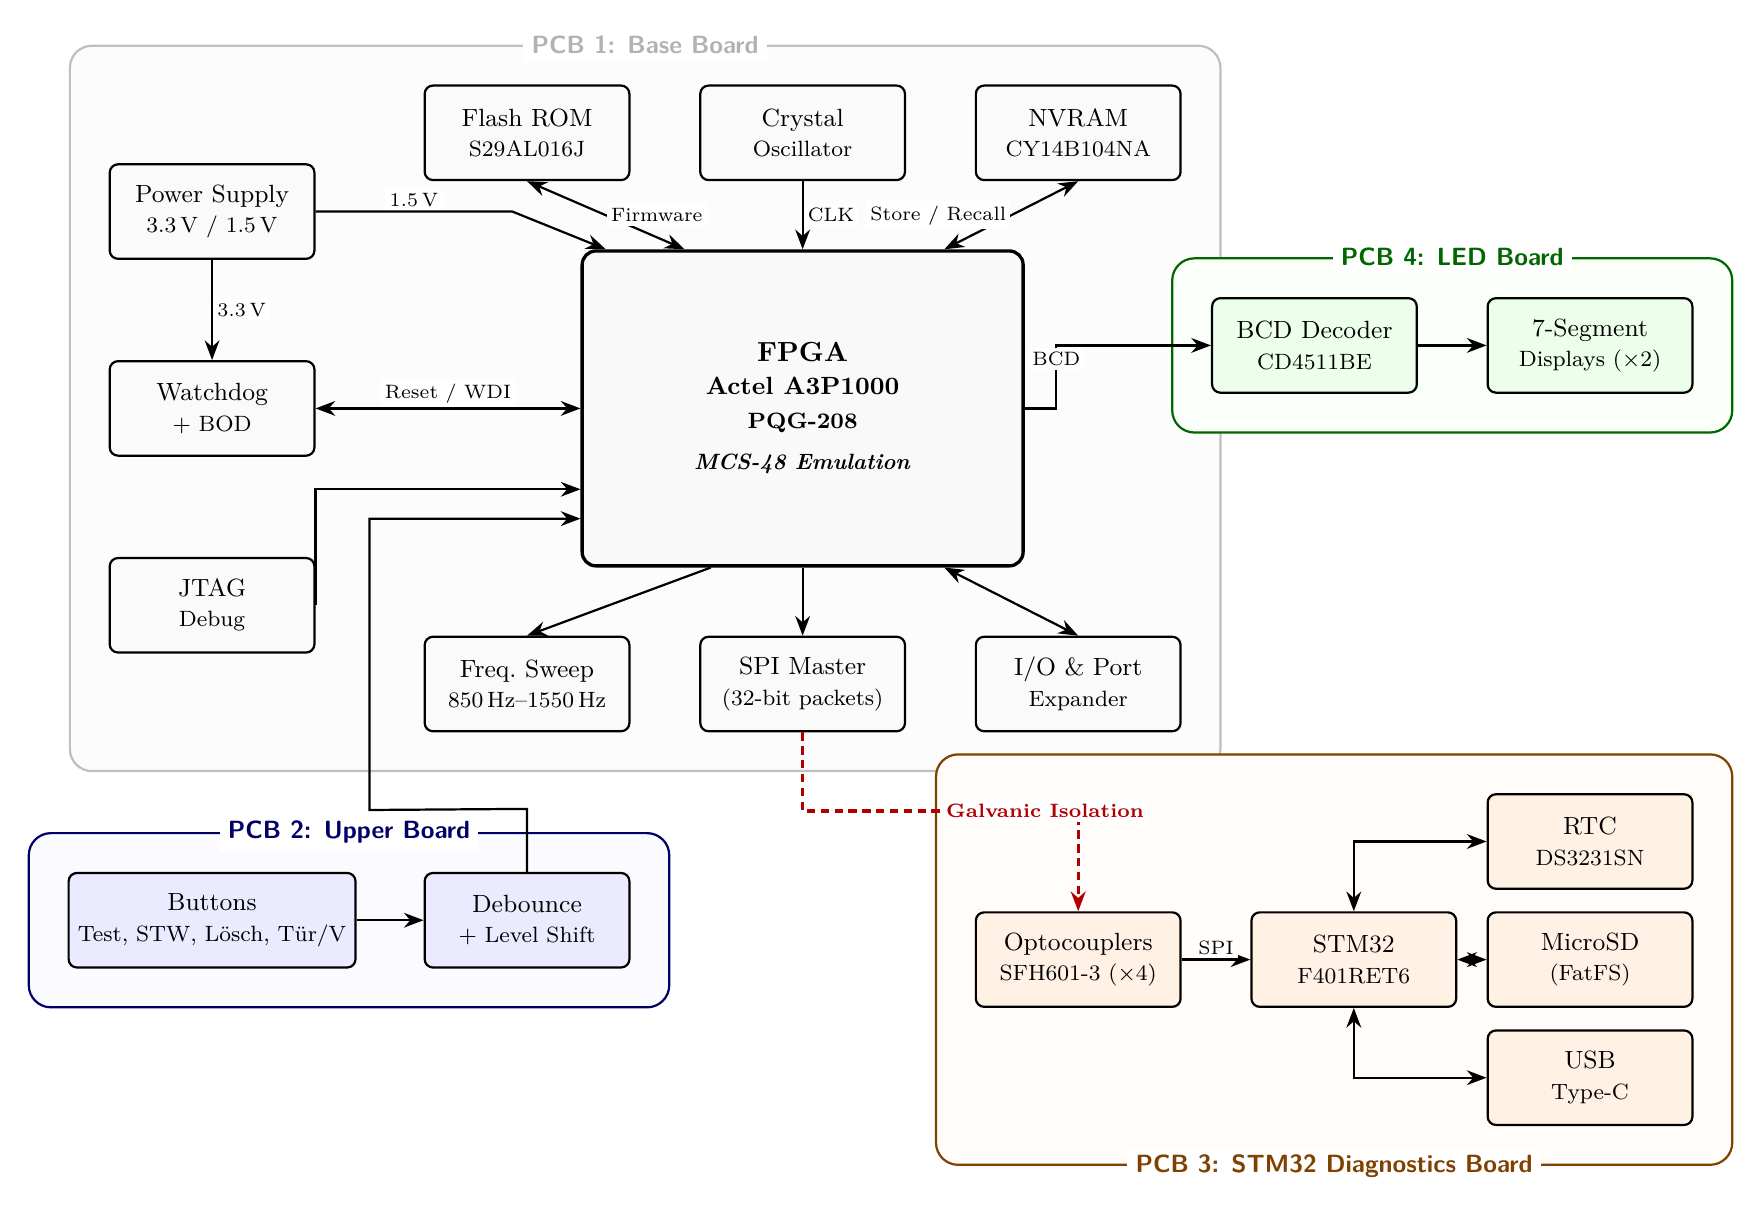
\begin{tikzpicture}[
    module/.style={draw, thick, rounded corners=3pt, minimum width=2.6cm,
                   minimum height=1.2cm, align=center, font=\small},
    fpga/.style={draw, very thick, rounded corners=5pt, minimum width=5.6cm,
                 minimum height=4cm, align=center, font=\normalsize\bfseries,
                 fill=gray!5},
    pcb/.style={draw, thick, rounded corners=8pt, inner sep=14pt},
    pcblabel/.style={font=\small\bfseries\sffamily, fill=white, inner sep=3pt},
    conn/.style={-{Stealth[length=2.5mm]}, thick},
    bconn/.style={{Stealth[length=2.5mm]}-{Stealth[length=2.5mm]}, thick},
    isoconn/.style={-{Stealth[length=2.5mm]}, very thick, densely dashed, red!70!black},
    lbl/.style={font=\scriptsize, midway, fill=white, inner sep=1.5pt},
    busarr/.style={-{Stealth[length=2.5mm]}, thick, double, double distance=1.2pt},
  ]

    % ================================================================
    % FPGA Core (centre)
    % ================================================================
    \node[fpga] (fpga) at (0,0) {FPGA\\{\small Actel A3P1000}\\{\footnotesize PQG-208}\\[3pt]{\footnotesize\itshape MCS-48 Emulation\/}};

    % ================================================================
    % Base Board peripherals
    % ================================================================
    % Top row
    \node[module, fill=gray!4] (pwr)   at (-7.5, 2.5) {Power Supply\\{\footnotesize \SI{3.3}{\volt} / \SI{1.5}{\volt}}};
    \node[module, fill=gray!4] (flash) at (-3.5, 3.5) {Flash ROM\\{\footnotesize S29AL016J}};
    \node[module, fill=gray!4] (xtal)  at (0, 3.5)    {Crystal\\{\footnotesize Oscillator}};
    \node[module, fill=gray!4] (nvram) at (3.5, 3.5)  {NVRAM\\{\footnotesize CY14B104NA}};

    % Left column
    \node[module, fill=gray!4] (wdog)  at (-7.5, 0)   {Watchdog\\{\footnotesize + BOD}};
    \node[module, fill=gray!4] (jtag)  at (-7.5, -2.5){JTAG\\{\footnotesize Debug}};

    % Bottom row
    \node[module, fill=gray!4] (freq)  at (-3.5, -3.5){Freq.\ Sweep\\{\footnotesize \SI{850}{\hertz}--\SI{1550}{\hertz}}};
    \node[module, fill=gray!4] (spi)   at (0, -3.5)   {SPI Master\\{\footnotesize (32-bit packets)}};
    \node[module, fill=gray!4] (ioexp) at (3.5, -3.5) {I/O \& Port\\{\footnotesize Expander}};

    % ================================================================
    % LED Display Board (right of FPGA)
    % ================================================================
    \node[module, fill=green!8] (bcd)  at (6.5, 0.8)  {BCD Decoder\\{\footnotesize CD4511BE}};
    \node[module, fill=green!8] (disp) at (10, 0.8)   {7-Segment\\{\footnotesize Displays ($\times 2$)}};

    % ================================================================
    % Upper Board (bottom-left)
    % ================================================================
    \node[module, fill=blue!8] (btns)     at (-7.5, -6.5) {Buttons\\{\footnotesize Test, STW, L\"osch, T\"ur/V}};
    \node[module, fill=blue!8] (debounce) at (-3.5, -6.5) {Debounce\\{\footnotesize + Level Shift}};

    % ================================================================
    % STM32 Diagnostics Board (bottom-right, isolated)
    % ================================================================
    \node[module, fill=orange!10] (opto) at (3.5, -7)   {Optocouplers\\{\footnotesize SFH601-3 ($\times 4$)}};
    \node[module, fill=orange!10] (stm)  at (7, -7)     {STM32\\{\footnotesize F401RET6}};
    \node[module, fill=orange!10] (rtc)  at (10, -5.5)  {RTC\\{\footnotesize DS3231SN}};
    \node[module, fill=orange!10] (sd)   at (10, -7)    {MicroSD\\{\footnotesize (FatFS)}};
    \node[module, fill=orange!10] (usb)  at (10, -8.5)  {USB\\{\footnotesize Type-C}};

    % ================================================================
    % PCB grouping boxes (background)
    % ================================================================
    \begin{scope}[on background layer]
      \node[pcb, draw=gray!50, fill=gray!2,
            fit=(fpga)(pwr)(flash)(xtal)(nvram)(wdog)(jtag)(freq)(spi)(ioexp)] (bb) {};
      \node[pcb, draw=green!40!black, fill=green!2,
            fit=(bcd)(disp)] (lb) {};
      \node[pcb, draw=blue!40!black, fill=blue!2,
            fit=(btns)(debounce)] (ub) {};
      \node[pcb, draw=orange!50!black, fill=orange!2,
            fit=(opto)(stm)(rtc)(sd)(usb)] (sb) {};
    \end{scope}

    % PCB labels (on top edge of each group)
    \node[pcblabel, text=gray!60] at (bb.north) {PCB 1: Base Board};
    \node[pcblabel, text=green!40!black] at (lb.north) {PCB 4: LED Board};
    \node[pcblabel, text=blue!40!black] at (ub.north) {PCB 2: Upper Board};
    \node[pcblabel, text=orange!50!black] at (sb.south) {PCB 3: STM32 Diagnostics Board};

    % ================================================================
    % Connections
    % ================================================================
    % Power – 1.5 V rail: horizontal east then down to FPGA top-left
    \draw[conn] (pwr.east) -- node[lbl, above] {\SI{1.5}{\volt}} ++(2.5,0) -- ([xshift=-2.5cm]fpga.north);
    \draw[conn] (pwr.south) -- node[lbl, right] {\SI{3.3}{\volt}} (wdog.north);

    % Watchdog ↔ FPGA
    \draw[bconn] (wdog.east) -- node[lbl, above] {Reset / WDI} (fpga.west);

    % JTAG → FPGA  (orthogonal: horizontal then vertical)
    \draw[conn] (jtag.east) |- (fpga.200);

    % Flash ROM ↔ FPGA – straight down from Flash to FPGA top
    \draw[bconn] (flash.south) -- node[lbl, right] {Firmware} ([xshift=-1.5cm]fpga.north);

    % Crystal → FPGA
    \draw[conn] (xtal.south) -- node[lbl, right] {CLK} (fpga.north);

    % NVRAM ↔ FPGA
    \draw[bconn] (nvram.south) -- node[lbl, left] {Store / Recall} ([xshift=1.8cm]fpga.north);

    % Freq sweep
    \draw[conn] (fpga.240) -- (freq.north);

    % SPI
    \draw[conn] (fpga.south) -- (spi.north);

    % I/O expander
    \draw[bconn] ([xshift=1.8cm]fpga.south) -- (ioexp.north);

    % BCD → displays
    \draw[conn] (fpga.east) -- ++(0.4, 0) |- node[lbl, above, pos=0.3] {BCD} (bcd.west);
    \draw[conn] (bcd.east) -- (disp.west);

    % Buttons → Debounce → FPGA  (orthogonal route wide-left of Freq. Sweep)
    \draw[conn] (btns.east) -- (debounce.west);
    \draw[conn] (debounce.north) -- ++(0,0.8) -- (-5.5,-5.1) -- (-5.5,-1.4) -- ([yshift=-1.4cm]fpga.west);

    % === Galvanic isolation boundary (orthogonal route) ===
    \draw[isoconn] (spi.south) -- ++(0,-1) -| node[lbl, right, text=red!70!black, font=\scriptsize\bfseries, pos=0.25] {Galvanic Isolation} (opto.north);
    \draw[conn] (opto.east) -- node[lbl, above] {SPI} (stm.west);

    % STM32 peripherals (clean orthogonal fan-out)
    \draw[bconn] (stm.north) |- (rtc.west);
    \draw[bconn] (stm.east) -- (sd.west);
    \draw[bconn] (stm.south) |- (usb.west);
  \end{tikzpicture}
  }%
  \caption{High-level block diagram of the retrofitted test-diagnosis system. Four \PCB{} modules are shown: the Base Board with the \FPGA{} core (grey), the Upper Board with operator controls (blue), the LED Board (green), and the galvanically isolated STM32 Diagnostics Board (orange). The dashed red line marks the safety isolation boundary.}
  \label{fig:system_overview}
\end{figure*}

\subsection{Base Board (\FPGA{} Core)}
The central hub houses the Actel A3P1000-PQG208 \FPGA{}, chosen for its flash-based non-volatile configuration, which is inherently immune to the configuration-memory upsets (firm errors) that affect SRAM-based alternatives~\cite{latifshabgahi2009redundancy}. The \FPGA{} runs an MCS-48 emulation core (the OpenCores \texttt{t48\_core}, integrated unmodified) executing the original \SI{2}{\kilo\byte} firmware binary from external flash ROM, thereby preserving the legacy control logic. In functional safety terms, this binary is pre-existing software of uncertain pedigree; its reuse is argued on the basis of its extensive field-operation history, analogous to the IEC~61508 proven-in-use route, while acknowledging that the statistical operational evidence that route formally requires lies beyond the present scope. Key peripherals emulated in \VHDL{} include:
\begin{itemize}
  \item Memory interfaces to Flash ROM (S29AL016J) and \NVRAM{} (CY14B104NA) for persistent fault code storage.
  \item 7-segment display driving logic via \BCD{}-to-7-segment decoders (CD4511BE).
  \item A digital frequency sweep generator, replacing the legacy analog voltage-controlled oscillator (VCO). The generator employs a division counter logic that translates the \SI{6}{\mega\hertz} system clock to an output frequency $f_{\text{out}}$ according to the relation:
  \begin{equation}
    f_{\text{out}}(i) = \frac{f_{\text{clk}}}{2 \cdot N_{\text{div}}(i)},
  \end{equation}
  where $f_{\text{clk}} = \SI{6}{\mega\hertz}$, and $N_{\text{div}}(i)$ is a clock division factor retrieved from a lookup table (LUT) implementing a non-linear sweep profile stepped by an internal \SI{600}{\hertz} clock. The division factor $N_{\text{div}}$ varies between $1935$ (yielding $f_{\text{out}} \approx \SI{1550.4}{\hertz}$) and $3529$ (yielding $f_{\text{out}} \approx \SI{850.1}{\hertz}$), covering the required diagnostic range of \SI{850}{\hertz} to \SI{1550}{\hertz} across 33 steps (up-sweep) and 65 steps (down-sweep), reproducing the asymmetric step granularity of the legacy sweep profile.
  \item An \SPI{} master for diagnostic data transmission to the STM32 subsystem.
  \item Watchdog interaction logic with an independent external hardware watchdog.
\end{itemize}

The board also integrates power regulation (TPS73615 and TPS73633), brown-out detection (\BOD{}) supervision via TPS3307, and a \JTAG{} interface for programming and boundary-scan testing.

\subsection{Upper Board (Legacy Interface)}
This module interfaces with the legacy system's mechanical buttons (Test, Control~[STW], Clear~[L\"osch], Door/Speed~[T\"ur/V]) through debouncing and level-shifting circuitry, preserving the original user interaction paradigm.

\subsection{STM32 Diagnostics Board}
A dedicated STM32F401RET6 (Arm Cortex-M4) provides enhanced logging capabilities, \textit{intentionally decoupled} from the safety-critical core through galvanic isolation. Four optocouplers (SFH601-3) isolate the \SPI{} communication link, with separate isolated DC/DC converters maintaining the power barrier. To ensure reliable signal transmission across the isolation boundary, the \FPGA{}'s emulated \SPI{} master clock frequency is set to $f_{\text{SPI}} = \SI{100}{\kilo\hertz}$ by division of the \SI{6}{\mega\hertz} system clock (30 clock cycles per half-period). The SFH601-3 optocoupler specifies typical turn-on and turn-off switching times $t_{\text{on}} \approx t_{\text{off}} \approx \SI{3}{\micro\second}$ (at $V_{\text{CC}} = \SI{5}{\volt}$, $I_C = \SI{2}{\milli\ampere}$, $R_L = \SI{100}{\ohm}$). Relative to the half-period, each switching edge therefore consumes a nominal margin of:
\begin{equation}
  t_{\text{margin}} = t_{\text{half}} - t_{\text{sw}} = \SI{5}{\micro\second} - \SI{3}{\micro\second} = \SI{2}{\micro\second},
\end{equation}
so the \SI{100}{\kilo\hertz} rate keeps each \SI{10}{\micro\second} bit period comfortably above the combined edge-switching time under typical operating conditions. The subsystem features an \RTC{} (DS3231SN) with battery backup for timestamped logging, a Secure Digital I/O (\SDIO{}) interface for MicroSD persistent storage, and \USB{} Type-C for data retrieval. While providing rich diagnostic data, the introduction of \USB{} and \SDIO{} interfaces expands the system's attack surface, necessitating future cybersecurity assessment aligned with IEC~62443~\cite{iec62443_2013}. Similar diagnostic and logging architectures have been surveyed in rolling stock applications~\cite{chen2020diagnostics}.

\subsection{LED Display Board}
Two Kingbright SC03-12EWA 7-segment displays, driven by CD4511BE decoders, provide visual fault code and self-test feedback to operators.

\subsection{Safety-Relevant Design Features}
Key safety features include: (1)~an independent hardware watchdog forcing system reset upon \FPGA{} hang detection, (2)~\BOD{} supervision on all critical power rails (\SI{5}{\volt}, \SI{3.3}{\volt}, \SI{1.5}{\volt}), (3)~galvanic isolation preventing fault propagation from non-safety (STM32) to safety (\FPGA{}) domains, and (4)~retention of legacy built-in self-test capabilities.

% =========================================================================
% IV. VERIFICATION METHODOLOGY
% =========================================================================
\section{Verification Methodology}
\label{sec:methodology}

\subsection{Two-Layer Verification Strategy}
The verification strategy combines structural (white-box) component testing with functional (black-box) system validation, structured around the V-model~\cite{iec61508_2010,en50716_2023} and IEEE~1012~\cite{ieee1012_2024}. Combining white-box and black-box testing throughout the V-model is standard software-engineering practice; this work adapts those complementary principles to a hardware/firmware retrofit. The two-layer design is necessary because verifying a new hardware core (the \FPGA{}) while validating its functional equivalence against a legacy microcontroller's behaviour introduces both physical and logical integration challenges that a single testing paradigm cannot resolve. As shown in Fig.~\ref{fig:v_model}, the methodology maps to the right side of the V-model through two layers:

\begin{figure}[!t]
  \centering
  \resizebox{\columnwidth}{!}{%
  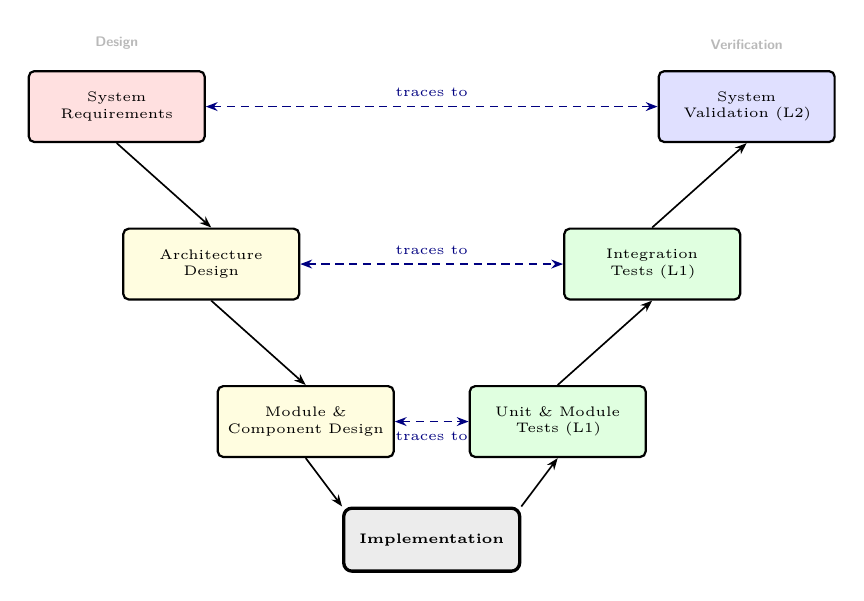
\begin{tikzpicture}[
    box/.style={draw, thick, rounded corners=2pt, text width=2.0cm,
                minimum height=0.9cm, align=center, font=\tiny},
    impl/.style={draw, very thick, rounded corners=3pt, text width=2.0cm,
                 minimum height=0.8cm, align=center, font=\tiny\bfseries,
                 fill=gray!15},
    hdr/.style={font=\tiny\bfseries\sffamily, text=gray!55},
    arr/.style={-{Stealth[length=1.5mm]}, semithick},
    darr/.style={{Stealth[length=1.5mm]}-{Stealth[length=1.5mm]}, semithick,
                 densely dashed, blue!50!black},
  ]
    % === V-model geometry (compact to fit IEEE column) ===
    % Left arm (Design, descending)
    \node[box, fill=red!12] (sr) at (0, 0)
      {System\\Requirements};
    \node[box, fill=yellow!12] (ad) at (1.2, -2)
      {Architecture\\Design};
    \node[box, fill=yellow!12] (md) at (2.4, -4)
      {Module \&\\Component Design};

    % Bottom apex (Implementation)
    \node[impl] (im) at (4, -5.5)
      {Implementation};

    % Right arm (Verification, ascending)
    \node[box, fill=green!12] (ut) at (5.6, -4)
      {Unit \& Module\\Tests (L1)};
    \node[box, fill=green!12] (it) at (6.8, -2)
      {Integration\\Tests (L1)};
    \node[box, fill=blue!12] (sv) at (8, 0)
      {System\\Validation (L2)};

    % Column headers
    \node[hdr, above=4pt of sr] {Design};
    \node[hdr, above=4pt of sv] {Verification};

    % === Arrows: design flow (left arm down) ===
    \draw[arr] (sr.south) -- (ad.north);
    \draw[arr] (ad.south) -- (md.north);
    \draw[arr] (md.south) -- (im.north west);

    % === Arrows: verification flow (right arm up) ===
    \draw[arr] (im.north east) -- (ut.south);
    \draw[arr] (ut.north) -- (it.south);
    \draw[arr] (it.north) -- (sv.south);

    % === Traceability arrows (horizontal dashed) ===
    \draw[darr] (sr.east) -- node[above, font=\tiny, text=blue!50!black] {traces to} (sv.west);
    \draw[darr] (ad.east) -- node[above, font=\tiny, text=blue!50!black] {traces to} (it.west);
    \draw[darr] (md.east) -- node[below, font=\tiny, text=blue!50!black] {traces to} (ut.west);
  \end{tikzpicture}
  }%
  \caption{Mapping of the two-layer verification strategy to the V-model.
  Layer~1 (green, L1) covers deterministic component and interface tests;
  Layer~2 (blue, L2) covers system-level black-box validation.}
  \label{fig:v_model}
\end{figure}

\begin{itemize}[nosep]
  \item \textbf{Layer~1 (Component \& Interface Tests):} maps to \textit{unit and integration testing}---deterministic, white-box verification proving that individual design artifacts (\VHDL{} modules, hardware interfaces) are correctly implemented against their technical specifications.
  \item \textbf{Layer~2 (System-Level Tests):} maps to \textit{system and acceptance testing}---black-box validation of the fully integrated system against original functional requirements (legacy system behaviour).
\end{itemize}

This combination---structural rigour at the component level (Layer~1) and functional fidelity at the integrated system level (Layer~2)---provides broader verification coverage than either technique in isolation.\looseness=-1

\subsection{Layer 1: Deterministic Component Verification}
\label{sec:layer1}

Layer~1 employed three complementary techniques:

\textbf{1) \VHDL{} Simulation:} Extensive pre- and post-synthesis simulations using ModelSim~ME verified the \FPGA{} design prior to hardware deployment. Dedicated testbenches provided controlled stimuli to verify: the emulated MCS-48 core behaviour, memory interface timing against component datasheet specifications (Flash ROM, \NVRAM{}), peripheral logic (display latching, button handling, frequency sweep, \SPI{} master), and watchdog interaction (Fig.~\ref{fig:watchdog}).

A critical finding during simulation was the discovery of the \NVRAM{} control logic bug: the \texttt{NVRAM\_ble} signal (the active-low byte-low-enable) was erroneously held at logic high in the inherited Rev~0.0 design, preventing correct access to the non-volatile memory~\cite{savchuk2025}. This defect had remained undetected through previous development phases because the \NVRAM{} was only exercised during fault storage and recall sequences---functions that were never systematically tested in isolation prior to this work. The fix was straightforward (permanently driving \texttt{NVRAM\_ble} low), but its discovery illustrates the diagnostic value of dedicated component-level testbenches in catching design faults that persist through integration.

\begin{figure}[!t]
  \centering
  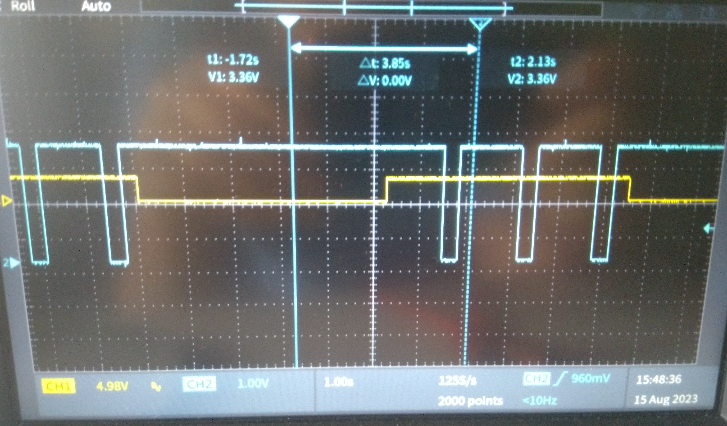
\includegraphics[width=\columnwidth]{watchdog_reaction.png}
  \caption{Oscilloscope capture from Layer~1 verification showing the watchdog circuit timing. CH1 (yellow): \FPGA{} servicing pulses. CH2 (blue): watchdog reset response.}
  \label{fig:watchdog}
\end{figure}

\textbf{2) Boundary Scan (\JTAG{}):} IEEE~1149.1 boundary scan confirmed \FPGA{} identification (A3P1000), successful bitstream programming, and I/O pin connectivity. This technique proved particularly valuable for diagnosing the approximately 40 \FPGA{} pins that required re-soldering: boundary scan could rapidly identify open or bridged connections without requiring functional firmware execution.

\textbf{3) Hardware Timing Measurements:} Oscilloscope measurements on the assembled Rev~1.0 hardware validated critical real-world timing parameters: watchdog pulse periodicity and the frequency sweep profile (\SI{850}{\hertz} to \SI{1550}{\hertz}). These measurements serve as the bridge between simulation-proven logical correctness and physical-world behaviour, confirming that the actual RC networks, crystal tolerances, and signal integrity meet design expectations.

\subsection{Layer 2: Fixture-Based System Validation}
\label{sec:layer2}

Layer~2 validated the fully integrated system using a dedicated hardware test fixture (``Testkartentester'')~\cite{dolata2023}. This layer addresses a fundamental limitation of Layer~1: simulation and hardware measurements verify individual components against their specifications, but cannot confirm that the complete system reproduces the legacy behaviour that operators and maintenance personnel rely on.

\textbf{Test Infrastructure:} The fixture (Fig.~\ref{fig:fixture}) provides physical connections via the main 48-pin DIN~41612 (type~F) system connector and interfaces with a host PC through an STM32 Nucleo-F401RE board. A Python application orchestrates test execution in a semi-automated workflow: it drives \GPIO{} pins to simulate fault conditions and system inputs, prompts the operator for manual checks (e.g., verifying 7-segment display codes visually), and logs pass/fail outcomes with timestamps. Each test scenario follows a four-phase cycle: (1)~stimulus application via pin control, (2)~settling delay (typically \SI{3}{\second} to match legacy button timing), (3)~expected-output assertion, and (4)~state cleanup via the L\"osch (clear) button.

\begin{figure}[!t]
  \centering
  \resizebox{\columnwidth}{!}{%
  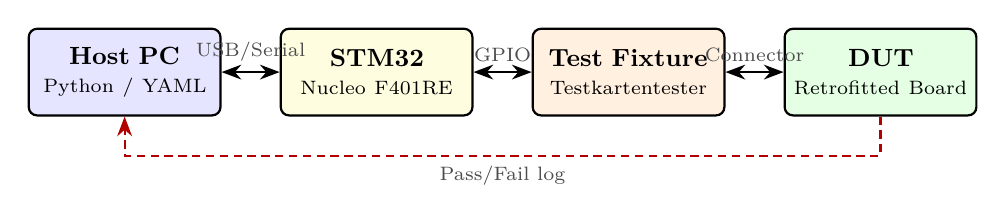
\begin{tikzpicture}[
    blk/.style={draw, thick, rounded corners=3pt, minimum height=1.1cm,
                align=center, font=\small, text width=2.2cm},
    arr/.style={-{Stealth[length=2.5mm]}, thick},
    barr/.style={{Stealth[length=2.5mm]}-{Stealth[length=2.5mm]}, thick},
    lbl/.style={font=\scriptsize, text=black!70, align=center},
  ]
    % Nodes -- left to right
    \node[blk, fill=blue!10]   (pc)   at (0,0)
      {\textbf{Host PC}\\[-1pt]{\scriptsize Python / YAML}};
    \node[blk, fill=yellow!12] (nuc)  at (3.2,0)
      {\textbf{STM32}\\[-1pt]{\scriptsize Nucleo F401RE}};
    \node[blk, fill=orange!12] (fix)  at (6.4,0)
      {\textbf{Test Fixture}\\[-1pt]{\scriptsize Testkartentester}};
    \node[blk, fill=green!10]  (dut)  at (9.6,0)
      {\textbf{DUT}\\[-1pt]{\scriptsize Retrofitted Board}};

    % Connections
    \draw[barr] (pc.east)  -- node[above, lbl] {USB/Serial} (nuc.west);
    \draw[barr] (nuc.east) -- node[above, lbl] {GPIO}       (fix.west);
    \draw[barr] (fix.east) -- node[above, lbl] {Connector}  (dut.west);
    \draw[arr, densely dashed, red!70!black]
          (dut.south) -- ++(0,-0.5) -| node[below, lbl, pos=0.25]
          {Pass/Fail log} (pc.south);
  \end{tikzpicture}
  }%
  \caption{Layer~2 test infrastructure. The PC orchestrates YAML-defined scenarios via an STM32 Nucleo board and the dedicated test fixture, which stimulates and monitors the Device Under Test~(DUT).}
  \label{fig:fixture}
\end{figure}

\textbf{YAML-Based Scenarios:} Test procedures were defined in YAML format, specifying: input pin stimuli (\texttt{pin\_sets}), expected display codes (\texttt{expected\_err\_code}), expected stored fault sequences (\texttt{expected\_err\_seq}), and required tester actions. This format ensures repeatability and provides implicit traceability to legacy requirements~\cite{rexroth1992wsp}.

\textbf{Coverage:} The test suite covered: (1)~complete fault memory cycles (trigger $\rightarrow$ display $\rightarrow$ store $\rightarrow$ recall $\rightarrow$ clear) for all documented fault codes, (2)~self-test activation and frequency sweep, (3)~button interaction equivalence, (4)~power-cycle stability, and (5)~diagnostic \SPI{} transmission to the STM32 logger.

Listing~\ref{lst:yaml} illustrates a representative two-step test scenario for a ``Geber~3'' (sensor fault on axle card~3). The first step triggers the fault via \texttt{pin\_sets}, asserts the expected immediate display code (\texttt{31}) and stored fault sequence (\texttt{03 31 09}). The second step verifies recall via the STW button and prompts the tester to clear the fault memory, confirming a complete storage-recall-clear cycle.

\begin{lstlisting}[language=YAML, caption={Example YAML test scenario: Geber~3 fault memory cycle.}, label={lst:yaml}, float=t]
# Geber 3 fault simulation (two-step sequence)
- name: Geber 3 - I
  description: >-
    Simulate sensor fault on axle 3. Wait 3 s for
    error display, then hold STW to verify sequence.
  pin_sets: {18z: 1, 24d: 0}
  expected_err_code: "31"
  expected_err_seq: "03 31 09"
  del: False

- name: Geber 3 - II
  description: Hold STW and verify stored sequence.
  pin_sets: {}
  expected_err_code: "95"
  expected_err_seq: "03 31 09"
  del: True   # Prompt tester to press 'Loesch'
\end{lstlisting}

\subsection{EN 50716 Modification Compliance}
\label{sec:en50716}

As a retrofit constitutes a modification, compliance with EN~50716~\cite{en50716_2023} was addressed through: \textit{impact analysis} (modification confined to hardware; safety-critical firmware unchanged), \textit{change verification} (the two-layer methodology itself), \textit{regression testing} (Layer~2 scenarios as a comprehensive regression suite), and \textit{configuration management} (Git version control for all artifacts).

% =========================================================================
% V. RESULTS AND DISCUSSION
% =========================================================================
\section{Results and Discussion}
\label{sec:results}

\subsection{Functional Equivalence Demonstration}

Functional equivalence of the safety-critical core was demonstrated through three converging lines of evidence:\looseness=-1

\begin{enumerate}[nosep]
  \item \textbf{Logical Correctness (\VHDL{} Simulation):} After correcting the \NVRAM{} control logic bug (\texttt{NVRAM\_ble}, the byte-low-enable, was erroneously held high~\cite{savchuk2025}), all Layer~1 simulations confirmed correct memory interface timing, peripheral logic behaviour, and watchdog interaction.
  \item \textbf{Physical Correctness (Hardware Measurement):} Post-rework oscilloscope measurements (Fig.~\ref{fig:watchdog}) confirmed critical timing parameters, including a watchdog service period of $\Delta t = \SI{3.85}{\second}$ at $V = \SI{3.36}{\volt}$ (against a nominal ${\approx}\,\SI{5}{\second}$ derived from the external watchdog's RC timing; the deviation is consistent with the tolerances of the timing components and comparator threshold, and with the idealised nature of the \VHDL{} timing model) and a validated frequency sweep from \SI{850}{\hertz} to \SI{1550}{\hertz}. This phase included extensive rework---approximately 40 \FPGA{} pins required re-soldering for stable operation~\cite{savchuk2025}.
  \item \textbf{Behavioural Equivalence (System Scenario Testing):} All Layer~2 test scenarios passed after resolving integration bugs. The test suite covered all 20 documented fault conditions (five categories---sensor fault, short circuit, wire break, monitoring timeout, and watchdog---across four axle cards), including complete fault memory cycles (trigger $\rightarrow$ display $\rightarrow$ store $\rightarrow$ recall $\rightarrow$ clear), the full self-test sequence with frequency sweep, all four operator button interactions (Test, STW, L\"osch, T\"ur/V), and power-cycle stability across multiple iterations.
\end{enumerate}

The convergence of these three independent lines of evidence---each addressing a distinct aspect of correctness (logical, physical, behavioural)---provides robust assurance of functional equivalence for the safety-critical core. Because this methodology relies on generic V-model principles and black-box I/O behaviour rather than system-specific knowledge, it can be adapted to other IEC~61508-compliant hardware retrofits.

Table~\ref{tab:results} provides a quantitative summary of all verification activities and their outcomes.

\begin{table}[!t]
  \centering
  \caption{Summary of verification results across both layers.}
  \label{tab:results}
  \scriptsize
  \setlength{\tabcolsep}{1pt}
  \begin{tabular*}{\columnwidth}{@{\extracolsep{\fill}}lllr@{}}
    \toprule
    \textbf{Test Category} & \textbf{Layer} & \textbf{Method} & \textbf{Result} \\
    \midrule
    Flash \& NVRAM timing       & L1 & ModelSim      & Pass \\
    Periph. logic (disp/sweep) & L1 & ModelSim    & Pass \\
    Watchdog interaction     & L1 & ModelSim         & Pass \\
    HW timing: watchdog      & L1 & Oscilloscope      & \SI{3.85}{\second} \\
    HW timing: sweep         & L1 & Oscilloscope      & \SI{850}{\hertz}--\SI{1550}{\hertz} \\
    JTAG scan                & L1 & Libero SoC        & Pass \\
    \midrule
    Faults (20 codes)           & L2 & Fixture/YAML & 20/20 \\
    Buttons (4 cases)           & L2 & Fixture/YAML & 4/4 \\
    Self-test                   & L2 & Fixture/YAML & Pass \\
    Power stability             & L2 & Fixture/YAML & Pass \\
    SPI (32-bit)                & L2 & Fixture/USB  & Pass$^*$ \\
    SD card                     & L2 & Firmware      & Pass$^\dagger$ \\
    \bottomrule
    \multicolumn{4}{@{}p{\linewidth}@{}}{\scriptsize $^*$Originally truncated to 16 bits; resolved by resizing the SPI reception buffer configuration to 32 bits (4 bytes) in the STM32 firmware.} \\
    \multicolumn{4}{@{}p{\linewidth}@{}}{\scriptsize $^\dagger$Originally blocked due to filesystem mounting delays; resolved by mounting once at initialization and optimizing the main logging loop.}
  \end{tabular*}
\end{table}

Fig.~\ref{fig:sweep_comparison} provides direct visual evidence of functional equivalence for the frequency sweep---a key anti-skid diagnostic function. The thin trend lines in both captures show close agreement between the original and emulated sweep profiles across the full \SI{850}{\hertz}--\SI{1550}{\hertz} range.

\begin{figure*}[!t]
  \centering
  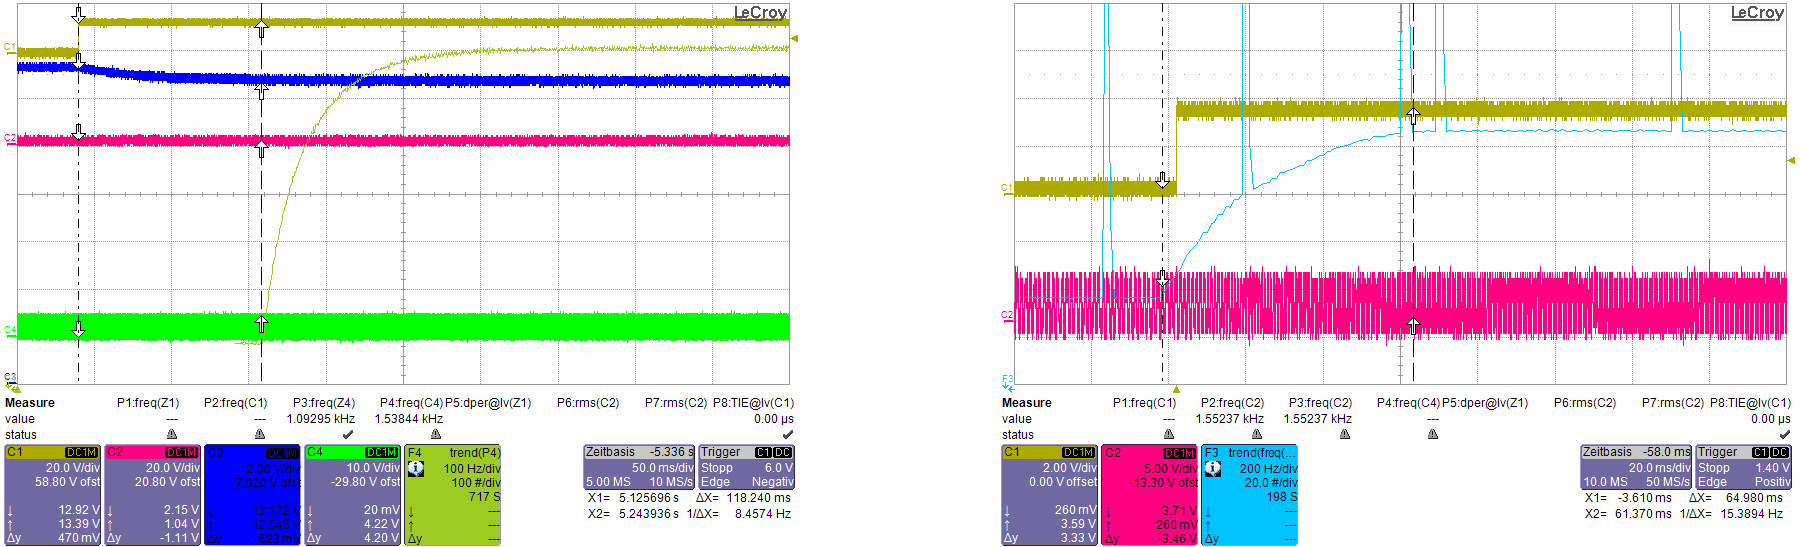
\includegraphics[width=0.49\textwidth]{comp_upsweep.png}%
  \hfill
  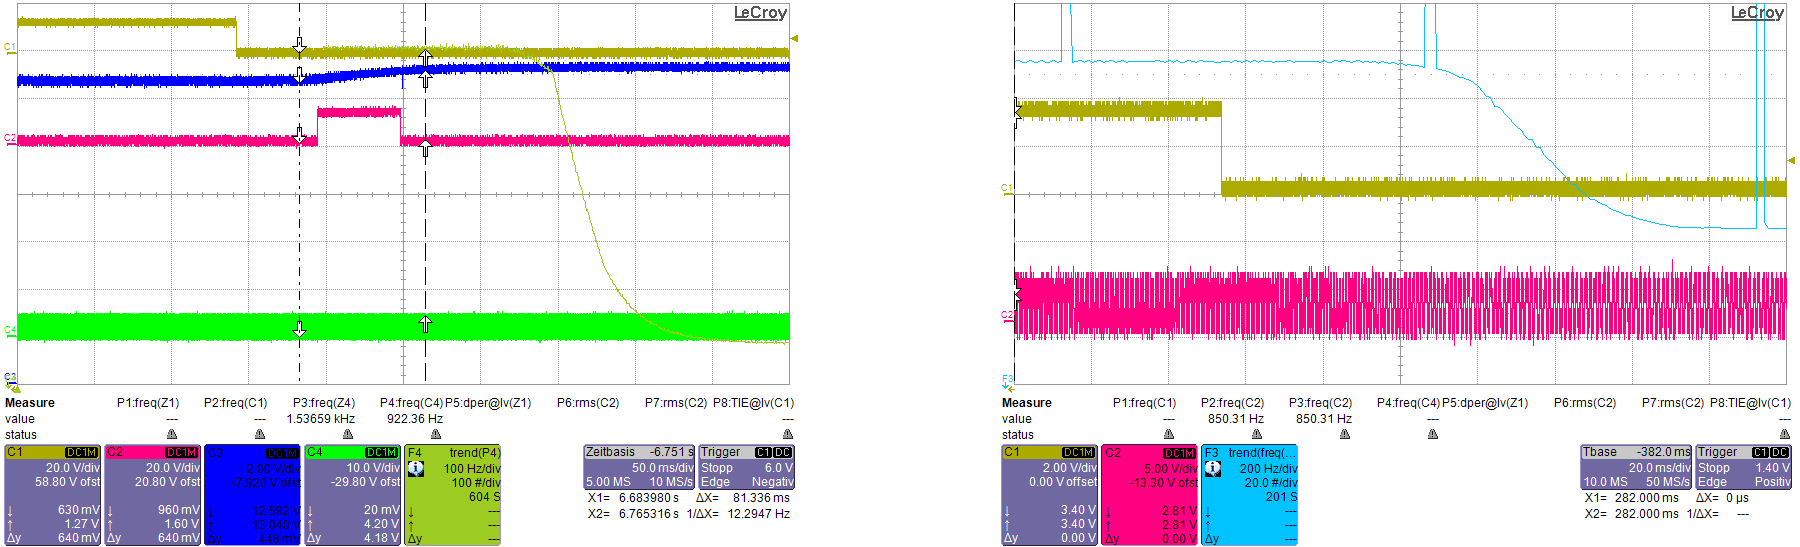
\includegraphics[width=0.49\textwidth]{comp_downsweep.png}
  \caption{Frequency sweep comparison: original system (left half of each panel, LeCroy oscilloscope) vs.\ FPGA emulation (right half). Left panel: ascending sweep (\SI{850}{\hertz}--\SI{1550}{\hertz}). Right panel: descending sweep (\SI{1550}{\hertz}--\SI{850}{\hertz}). The thin trend lines confirm matching frequency-response curves.}
  \label{fig:sweep_comparison}
\end{figure*}

\subsection{Verification Coverage and the Diagnostic Blind Spot}
\label{subsec:blind_spot_analysis}

The empirical validation of the retrofitted system on the target hardware revealed five distinct integration bugs across the hardware, firmware, and logical design domains, as categorized in Table~\ref{tab:bugs_matrix}. An analysis of these defects highlights the complementary nature of the two-layer framework: it applies the standard software-engineering V-model principle---structural component-level tests followed by functional system-level validation---to a hardware/firmware retrofit. The results demonstrate that neither verification layer alone is sufficient to ensure safety-critical functional equivalence.

\begin{table}[!t]
  \centering
  \caption{Taxonomic Classification of Discovered Integration Bugs.}
  \label{tab:bugs_matrix}
  \scriptsize
  \setlength{\tabcolsep}{1pt}
  \begin{tabular*}{\columnwidth}{@{\extracolsep{\fill}}llp{2.3cm}lll@{}}
    \toprule
    \textbf{ID} & \textbf{Class} & \textbf{Description} & \textbf{Layer} & \textbf{Instrument} & \textbf{Status} \\
    \midrule
    B1 & Logical & NVRAM byte-low-enable (\texttt{NVRAM\_ble}) held high & L1 & Simulation & Resolved \\
    B2 & Layout  & STM32 SWD debug pins routed incorrectly           & L1 & Boundary-Scan & Reworked \\
    B3 & Assembly& Approx. 40 FPGA pins open or shorted              & L1 & JTAG / Scope  & Reworked \\
    B4 & Firmware& FatFS timing starvation blocking SPI Rx           & L2 & Fixture/YAML  & Resolved \\
    B5 & Interface& SPI payload truncation (16-bit vs 32-bit buffer)  & L2 & Fixture/USB   & Resolved \\
    \bottomrule
  \end{tabular*}
\end{table}

Structural verification and boundary-scan diagnostics (Layer~1) isolated the NVRAM byte-low-enable error ($B_1$), the incorrect SWD pin routing ($B_2$), and the FPGA solder-joint assembly defects ($B_3$). However, because Layer~1 lacks a dynamic runtime integration environment, it could not expose firmware-level timing starvation ($B_4$) or SPI buffer truncation ($B_5$).

Conversely, system-level validation using the dedicated test fixture (Layer~2) stimulated the system through its external connector pins and captured the runtime integration errors $B_4$ and $B_5$. However, Layer~2 is constrained by observational limits: during functional testing, the internal RAM cache temporarily satisfied transient read/write commands, rendering the inactive NVRAM ($B_1$) latent and invisible at the external board boundary. Similarly, the physical assembly faults ($B_3$) caused intermittent crashes that could not be isolated or root-caused without Layer~1 boundary-scan tools.

Thus the two layers are mutually reinforcing: Layer~1 verifies structural correctness and exposes latent faults that escape functional testing, while Layer~2 validates real-time dynamic behaviour and exposes timing or protocol mismatches that component simulation cannot capture. Their convergence provides the verification coverage required for safety-critical retrofits.

\subsection{Safety Compliance}

Table~\ref{tab:standards} summarises how the methodology maps to applicable standards. Layer~1 tests trace to HDL module requirements from reverse engineering; Layer~2 YAML scenarios trace to legacy functional requirements~\cite{rexroth1992wsp}. The generated artifacts under Git version control establish the evidence base for formal safety assessment. For certification, these implicit traceability links would need to be formalised into explicit requirements-to-test matrices.\looseness=-1

\begin{table}[!t]
  \centering
  \caption{Standards compliance mapping for the two-layer verification methodology.}
  \label{tab:standards}
  \footnotesize
  \setlength{\tabcolsep}{4pt}
  \begin{tabular}{@{}lll@{}}
    \toprule
    \textbf{Standard} & \textbf{Scope} & \textbf{Layer} \\
    \midrule
    IEC~61508~\cite{iec61508_2010} & Safety lifecycle, SIL & L1 + L2 \\
    EN~50129~\cite{en50129_2018}   & HW safety evidence     & L1 + L2 \\
    EN~50716~\cite{en50716_2023}   & SW modification         & L1 + L2 \\
    EN~50155~\cite{en50155_2021}   & Environmental req.      & Future \\
    EN~61373~\cite{en61373_2010}   & Shock \& vibration       & Future \\
    IEEE~1012~\cite{ieee1012_2024} & V\&V process             & L1 + L2 \\
    \bottomrule
  \end{tabular}
\end{table}

\subsection{Diagnostic Subsystem Validation}

After re-routing the STM32 Serial Wire Debug (SWD) pins and debugging the firmware state machine~\cite{savchuk2025}, diagnostic data routing was validated via \USB{} serial streaming, confirming isolation integrity, error-free 32-bit \SPI{} packet reception, and robust SD logging.

\subsection{Resolved Integration Issues}
\label{sec:limitations}

The discovery of the following integration issues during Layer~2 testing validates the necessity of the scenario-based approach; these faults would not have been detected by Layer~1 simulation alone. To preserve safety integrity, these issues were subsequently resolved:
\begin{itemize}[nosep]
  \item \textbf{SD Card Storage (FatFS Timing Starvation):} The FatFS implementation on the STM32 initially caused firmware timing starvation during block write attempts to the MicroSD card. Root-cause analysis revealed that the firmware unconditionally mounted and unmounted the filesystem volume on every write loop cycle, which introduced a \SIrange{50}{200}{\milli\second} blocking overhead. This file system overhead, combined with blocking delays in the main execution thread, starved the SPI receive interrupt re-arming window, resulting in data overruns. This was resolved by mounting the SD card once at initialization, removing the loop-level mounting calls, and reducing the logging frequency.
  \item \textbf{\SPI{} Payload Truncation and Alignment:} The VHDL SPI master correctly transmits a 32-bit diagnostic frame (consisting of a 2-bit event-type prefix, 6-bit button state, and 24-bit error code). However, the STM32 firmware was initially misconfigured to receive only 16 bits per transaction (\texttt{HAL\_SPI\_Receive\_IT} was called with a buffer size of 2). This mismatch truncated the payload and left the remaining 16 bits unread. The leftover clock pulses triggered a receiver buffer overrun (\texttt{OVR} flag in the SPI status register) and caused persistent frame misalignment on subsequent transfers. Correcting the STM32 RX buffer size configuration to 32 bits (4 bytes) resolved the truncation and misalignment.
  \item \textbf{Residual Scope Gaps:} Formal methods (e.g., model checking, equivalence checking), quantitative structural coverage metrics (statement/branch coverage for VHDL), accredited environmental testing (EN~50155~\cite{en50155_2021}, EN~61373~\cite{en61373_2010}), and full \HIL{} integration with the complete braking system were beyond project scope. These activities are required for formal safety certification and are identified as future work.
\end{itemize}

Crucially, both the SPI bug and the FatFS issue reside exclusively in the non-safety-critical diagnostic subsystem, which is galvanically isolated from the \FPGA{} core. They do not affect the equivalence demonstration of the safety-critical functions verified through Layers~1 and~2 (see Sections~\ref{sec:layer1} and~\ref{sec:layer2}). This architectural separation---enforced by optocoupler isolation and independent power domains---ensures that diagnostic subsystem faults cannot propagate to the safety-critical domain. Board-level retrofits also avoid the embodied emissions of manufacturing replacement subsystems, consistent with broader rail-sector decarbonisation efforts~\cite{carbon_infra_uic_2016}.

% =========================================================================
% VI. CONCLUSION AND FUTURE WORK
% =========================================================================
\section{Conclusion}
\label{sec:conclusion}

This paper has proposed and validated a structured, two-layer verification methodology for demonstrating functional equivalence in safety-critical \FPGA{} retrofits, mapping standard V-model testing principles to the hardware/firmware integration domain. The central insight is that neither white-box simulation nor black-box system testing alone provides adequate coverage for modernising legacy safety hardware: simulation cannot expose physical integration defects, while system-level testing lacks the granularity to isolate fundamental logic errors. By orchestrating a layered convergence of evidence---grounded in the V-model and IEEE~1012---the methodology provides the diagnostic depth required to demonstrate functional equivalence with the original legacy system across the documented fault codes, self-test sequences, and user interactions.

The practical realities of stabilising an inherited prototype---the re-soldering of roughly 40 \FPGA{} pins alongside several firmware interventions---underline a key lesson for hardware retrofits: legacy migration should include a dedicated hardware-stabilisation phase, and design-for-debuggability should be a primary rather than secondary requirement. These findings are not specific to the anti-skid domain and apply to comparable safety-critical legacy-to-\FPGA{} modernisation efforts.

\textbf{Future work:} The immediate priority is to harden the diagnostic firmware beyond the stopgap fixes of Section~\ref{sec:limitations}---replacing them with a non-blocking, DMA-backed \SPI{} reception path and a logging queue decoupled from the receive interrupt. Longer-term objectives encompass full \HIL{} integration~\cite{hil_rail_suspension_2023,zhou_wu_2020}, cybersecurity assessment compliant with IEC~62443~\cite{iec62443_2013}, and the transition to professionally manufactured \PCB{}s for accredited environmental certification (EN~50155~\cite{en50155_2021}, EN~61373~\cite{en61373_2010}). Future work can formalise the proposed verification architecture into a generalised, certifiable framework for the sustainable modernisation of IEC~61508-compliant railway electronics.

% =========================================================================
% ACKNOWLEDGMENT
% =========================================================================
\section*{Acknowledgment}

The author thanks his supervisor for guidance throughout this research. The author also thanks S.~Ayoub, M.~Leyer, A.~Dolata, D.~Ostermann, F.~Schiffelers, D.~Savchuk, D.~C.~Icyer, E.~Galustian, and O.~Al-Selwi for their foundational and follow-on contributions to the hardware, firmware, and test fixture development.

% =========================================================================
% REFERENCES
% =========================================================================
\bibliographystyle{IEEEtran}
\bibliography{references}

\end{document}
